\section{SDHCAL}
\subsection{Collaborating Institutions}
Several CALICE groups are involved in the SDHCAL project but only LAPP is driving the R\&D for Micromegas calorimetry. Recently, some collaboration formed with other groups interested in the application of Micro Pattern Gaseous Detectors for calorimetry at a linear collider and at the HL-LHC:

\begin{itemize}
\item
Weizmann Institute of Science (Rehovot, Israel);
\item
the Institute of research into the fundamental laws of the Universe (Saclay, France);
\item
the Institute of Nuclear Particle Physics (Athens, Greece).
\end{itemize}

\subsection{Introduction}
The Micromegas R\&D pursued at LAPP is primarily intended for Particle Flow calorimetry at future linear colliders. It focuses on hadron calorimetry with large-area Micromegas segmented in very small readout cells of 1$\times$1\,cm$^{2}$. This granularity provides unprecedented imaging capability which can be exploited to improve the measurement of jet energy. Past and current R\&D efforts are described with emphasis on achievements since the publication of the ILC Detailed Baseline Design.
\subsection{Recent Milestones}


\subsubsection{The SDHCAL}

The SDHCAL is a prototype of imaging hadron calorimeter equipped with 50 layers of gaseous detectors of 1$\times$1\,m$^{2}$ interleaved by steel absorbers (Fig.\,\ref{sdhcal} (left)). Each detectors is segmented in pads of 1$\times$1\,cm$^{2}$ and the processed pad signal is coded over 2-bits (Fig.\,\ref{sdhcal} (right). The number of readout channels per layer imposes to integrated the front-end electronics directly on the gaseous detector printed-circuit-boards (PCB). Several CALICE groups are involved in this project. The LAPP group developed technologically advanced Micromegas prototypes in view of test in the SDHCAL. It also took responsibility of part of the data acquisition system (DAQ).


\begin{figure}
\begin{centering}
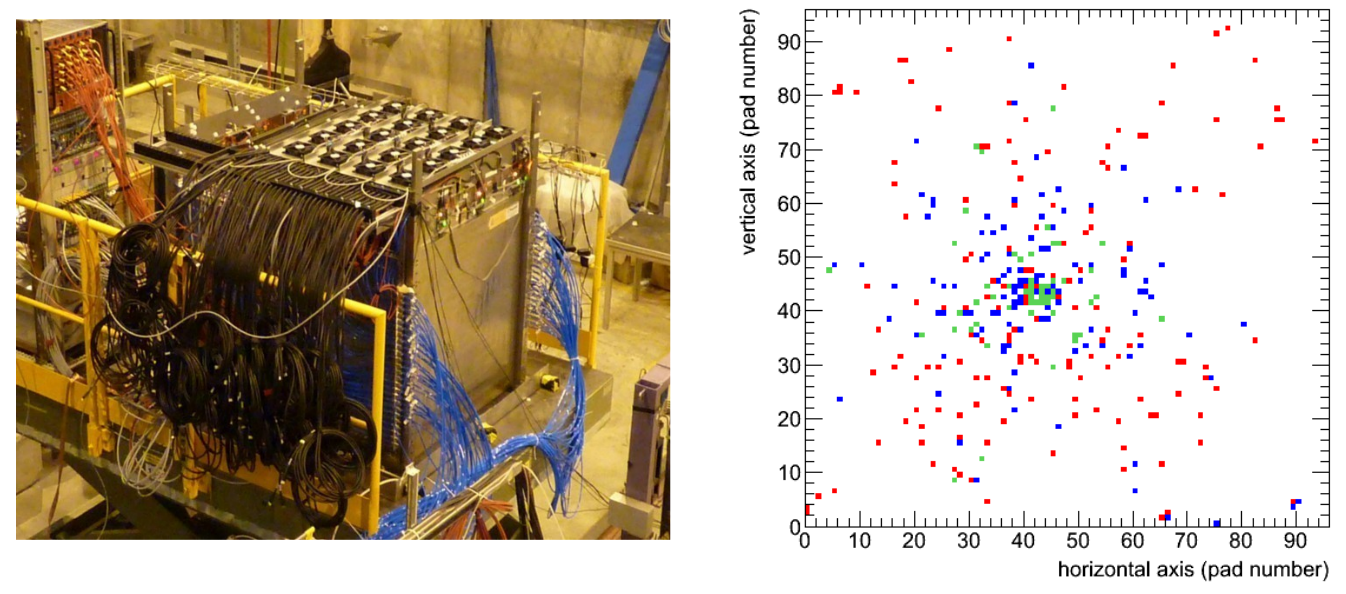
\includegraphics[width=0.95\textwidth]{Calorimeter/SDHCAL/test}
\caption{SDHCAL prototype in a beam line at the SPS at CERN (left). Event display of a 150\,GeV pion shower measured in a Micromegas prototype after 2\,$\lambda_{\rm int}$ of steel (right), the color indicates the threshold passed: red for 1, blue for 2 and green for 3.}
\label{sdhcal}
\end{centering}
\end{figure}


\subsubsection{The 1$\times$1\,m$^{2}$ Micromegas prototype}

\paragraph{Mechanics}
The Micromegas layers for the SDHCAL are made out of 6 high-voltage units installed together inside a gaseous chamber (Fig.\,\ref{mecha_elec} (right)). Each unit is an 8 layer PCB with a Bulk Micromegas mesh, readout pads and front-end ASICs; it is dubbed Active Sensor Unit (or ASU). A drift gap of 3\,mm is defined by spacers and a frame. Spacers are inserted in between ASUs, resulting in an inactive area of 2\,\%.


\begin{figure}
\begin{centering}
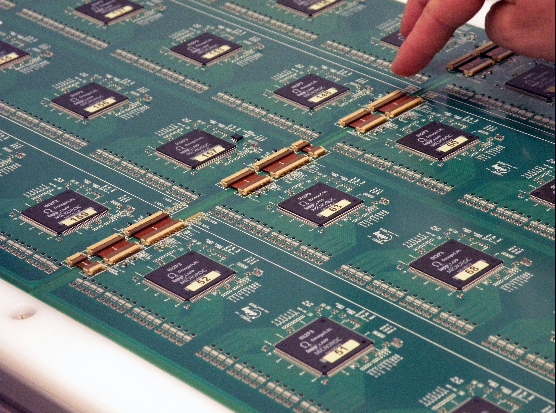
\includegraphics[width=0.45\textwidth]{Calorimeter/SDHCAL/intercon}
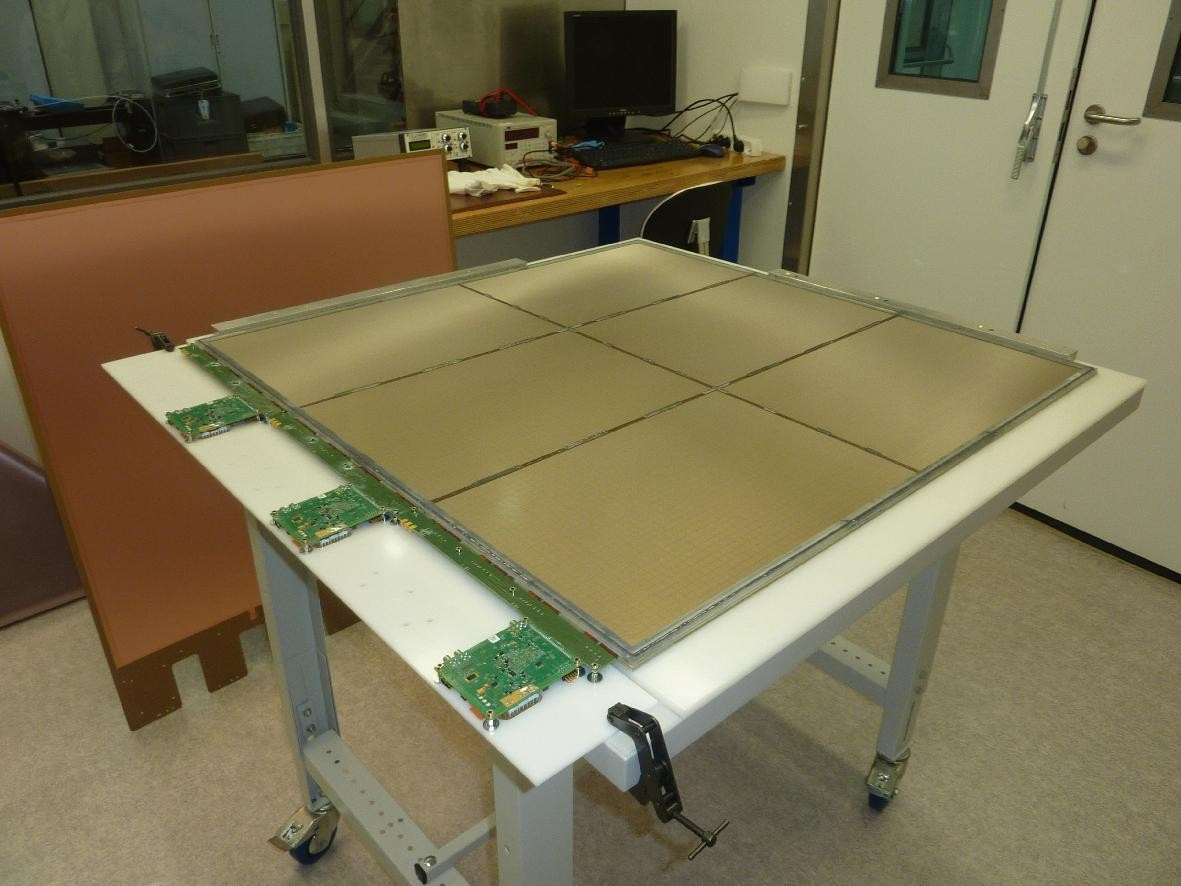
\includegraphics[width=0.45\textwidth]{Calorimeter/SDHCAL/m2_assembly}
\caption{Photographs of interconnections between 2 Active Sensor Units (left) and a 1$\times$1\,m$^{2}$ Micromegas prototype during assembly showing 6 of these units and a drift cover (right).}
\label{mecha_elec}
\end{centering}
\end{figure}


\paragraph{Electronics}
Electronics connections to the DAQ as well as services (power cables, gas pipes) are provided on one side of the prototype. ASU-to-ASU connections are therefore mandatory and are made with dedicated connectors and flexible cables (Fig.\,\ref{mecha_elec} (left)). They are used to distribute clocks and supply power to the ASICs, high voltage to the meshes, to configure the ASICs and read out data. Prior to assembly, 4 ASUs were chained and functional electronic tests were successfully performed. These key features make the design of the 1$\times$1\,m$^{2}$ Micromegas prototype fully scalable to the required size of a HCAL module at a future LC (at most 2\,m in the SiD detector concept).

\paragraph{Noise and detection efficiency}
A few prototypes were constructed~\cite{Adloff201390} and extensively tested in beam at CERN~\cite{Adloff:2014qea}. Noise conditions were excellent both during standalone tests and inside the CALICE SDHCAL. ASIC thresholds can be lowered down to about 20\,\% of a minimum ionising particle (MIP) signal at a typical running gas gain of 1500. Efficiency in excess of 95\,\% are easily reached while keeping a pad multiplicity below 1.1 for MIPs. The actual charge threshold is as low as 1--2\,fC; it is achieved on ASIC test-boards as well as once mounted on ASUs. The contribution of the PCB internal capacitances to the overall detector noise is therefore negligible.

\paragraph{Standalone performance}
Thanks to a precise control of the gas gaps and electronics settings, ASIC-to-ASIC variations of efficiency are below the percent in all tested prototypes. Although the statistics is low, the construction process seems reproducible. Stability with rate in high-energy hadron showers is excellent. Except occasional sparks, no effect of beam rate was observed on the pion response up to roughly 30 kHz beam rate; which was the highest rate during the tests. The measured spark probability lies in the range of 10$^{-6}$--10$^{-5}$ per showering pion at a running gas gain of 1500.

\subsubsection{Resistive prototypes}

While the Bulk Micromegas mesh is made of steel wires and is very resistant to sparking, sensitive front-end ASICs can suffer irreversible damage. Protections in the form of current-limiting diodes networks soldered on PCB were proved so far efficient. To simplify the PCB design and possibly reduce the overall detector cost, it is however desirable to get rid of diodes. It is well known that sparks can be suppressed by means of resistive coatings on the anode pad plane. This solution is used with great success in tracking detectors. Because it modifies the signal development, it needs some adaptation to calorimetry so as to preserve linearity and keep a narrow pad response function for Particle Flow reconstruction.


\begin{figure}
\begin{centering}
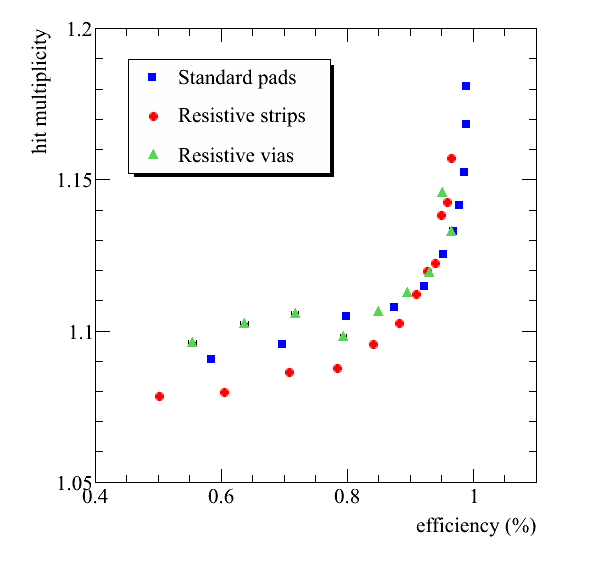
\includegraphics[width=0.45\textwidth]{Calorimeter/SDHCAL/splam_eff}
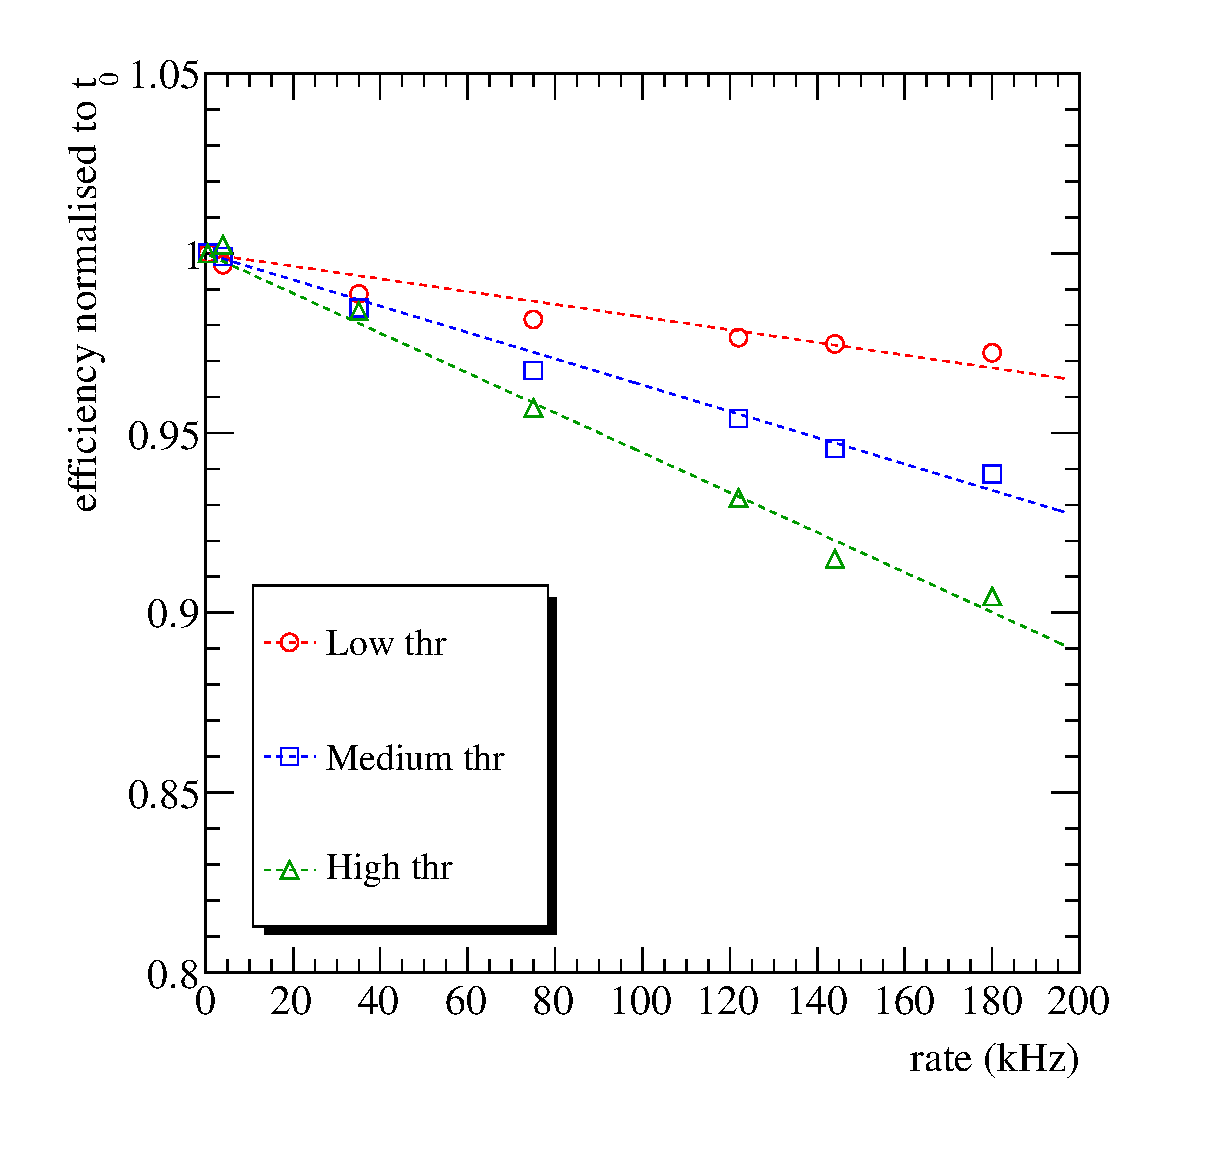
\includegraphics[width=0.45\textwidth]{Calorimeter/SDHCAL/splam_rate}
\caption{Pad multiplicity versus efficiency to 3\,GeV electrons for 2 resistive and 1 non-resistive (or standard) Micromegas prototypes (left). Efficiency dependence on rate in a resistive prototype for 3 values of threshold (right). The electron beam spot is $\sim$\,2$\times$2\,cm$^{2}$.}
\label{resistive}
\end{centering}
\end{figure}


First resistive designs using resistive strips and pads were implemented on small size prototypes. In a mixture of Ar/CO2, full suppression of sparking was demonstrated up to gas gain in excess of 10$^{4}$. At comparable gas gains, resistive and non-resistive prototypes show similar response to traversing charged particles, reaching high efficiency and low pad multiplicity. Compared to non-resistive ones, the evacuation of charge is slowed down in resistive prototypes which are thus subject to rate-dependent drops of gas gain. Expected efficiency losses have been observed at (3\,GeV electrons) rates in excess of 10\,kHz/cm$^{2}$. This limit is compatible with the resistivity of the coated material. At lower rates, it could be shown that the linearity of a Micromegas calorimeter to electrons is not affected by the resistive coatings, up to 5\,GeV, which was the maximum energy available during the testbeam campaign.

\subsection{Engineering Challenges}

\subsection{Future Plans}
Plans for the coming years include maintaining a commitment to linear collider detector R\&D and possibly seek new applications. Despite a decline of resources, an R\&D program to optimise resistive Micromegas for calorimetry is established. Linearity, rate capability and spark protection in dense electromagnetic showers will be checked up to high-energy and for detector designs with a large variety of resistivity and geometry. These measurements will be necessary to validate the resistive Micromegas technology for calorimetry at a future LC. Also, the on-going R\&D for high-luminosity LHC (HL-LHC) detector upgrades are an appealing perspective to the LAPP group. In particular, the possibility to equip the backing part of the CMS forward calorimeter is being investigated. Such high-rate application will put strong stability constraints on resistive Micromegas, making the optimisation work mentioned above even more relevant.

\begin{figure}
\begin{centering}
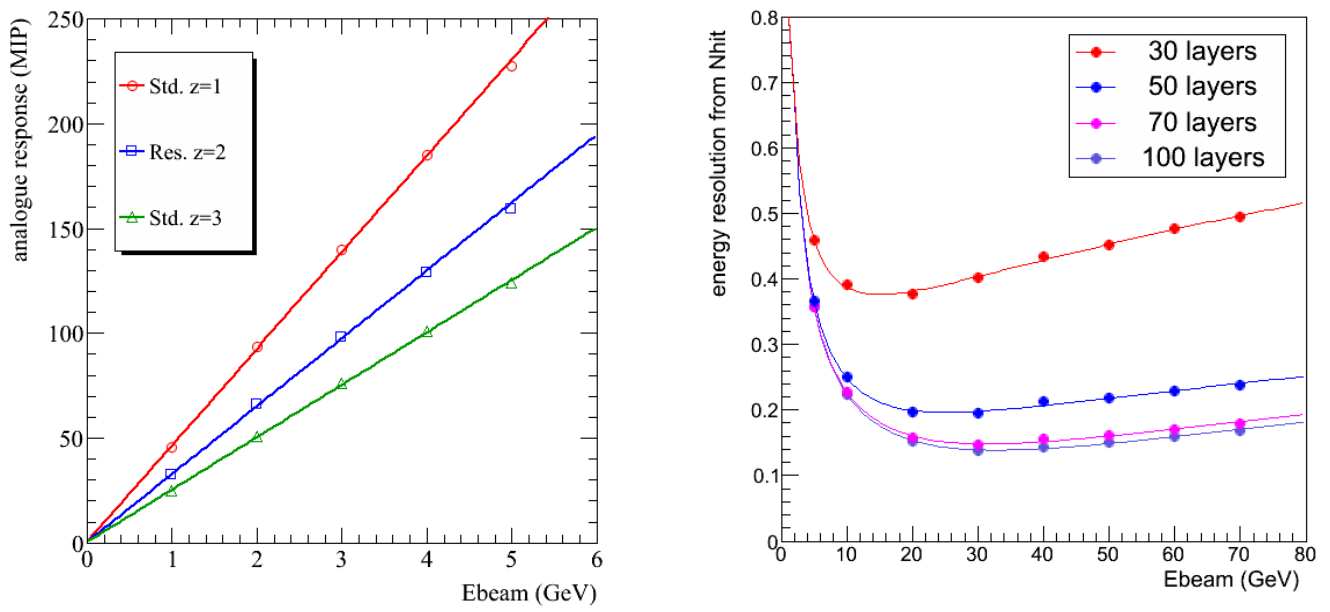
\includegraphics[width=0.8\textwidth]{Calorimeter/SDHCAL/test2}
\caption{Electron response of a virtual Micromegas SDHCAL deduced from measurements of longitudinal shower profiles in non-resistive (z=1 and z=3) and resistive (z=2) Micromegas prototypes placed behind increasing thicknesses of passive material (left). Geant4 calculation of the energy resolution to pions of a Micromegas DHCAL of 30 to 100 layers based on simple hit counting (right).}
\label{future}
\end{centering}
\end{figure}

On a longer term and if resources are sufficient, a Micromegas calorimeter prototype should be constructed so its performance can be compared to concurrent detector technologies. Some performance have already been studied with Monte Carlo simulation, the minimal prototype dimensions are known as well as its cost. This final step of the project naturally comes after optimisation of the resistive coating and would complete the R\&D on Micromegas calorimetry.

\subsection{Applications Outside of Linear Colliders}
